\documentclass[sigconf]{acmart}

\usepackage{hyperref}

%\usepackage{endfloat}
%\renewcommand{\efloatseparator}{\mbox{}} % no new page between figures

\usepackage{booktabs} % For formal tables

\settopmatter{printacmref=false} % Removes citation information below abstract
\renewcommand\footnotetextcopyrightpermission[1]{} % removes footnote with conference information in first column
\pagestyle{plain} % removes running headers

\usepackage{listings}
\usepackage{color}  

\lstset{ 
	language=R,                     % the language of the code
	basicstyle=\scriptsize\ttfamily, % the size of the fonts that are used for the code
	numbers=left,                   % where to put the line-numbers
	numberstyle=\tiny\color{blue},  % the style that is used for the line-numbers
	stepnumber=1,                   % the step between two line-numbers. If it is 1, each line
	% will be numbered
	numbersep=5pt,                  % how far the line-numbers are from the code
	backgroundcolor=\color{white},  % choose the background color. You must add \usepackage{color}
	showspaces=false,               % show spaces adding particular underscores
	showstringspaces=false,         % underline spaces within strings
	showtabs=false,                 % show tabs within strings adding particular underscores
	frame=single,                   % adds a frame around the code
	rulecolor=\color{white},        % if not set, the frame-color may be changed on line-breaks within not-black text (e.g. commens (green here))
	tabsize=2,                      % sets default tabsize to 2 spaces
	captionpos=b,                   % sets the caption-position to bottom
	breaklines=true,                % sets automatic line breaking
	breakatwhitespace=false,        % sets if automatic breaks should only happen at whitespace
	keywordstyle=\color{blue},      % keyword style
	commentstyle=\color{orange},   % comment style
	stringstyle=\color{red}      % string literal style
} 


\begin{document}
		
	\title{Predicting House Prices using Supervised Machine Learning Algorithms}
	
	
	\author{Murali Cheruvu, Anand Sriramulu}
	\orcid{xxxx-xxxx-xxxx}
	\affiliation{%
		\institution{Indiana University}
		\streetaddress{3209 E 10th St}
		\city{Bloomington} 
		\state{Indiana} 
		\postcode{47408}
	}
	\email{mcheruvu@iu.edu, asriramulu@iu.edu}
	
	% The default list of authors is too long for headers}
	\renewcommand{\shortauthors}{M. Cheruvu, A Sriramulu}
	
	
	\begin{abstract}
		
	Apply exploratory data analysis and linear regression, a supervised machine learning algorithm, to predict Sale Prices of list of homes found in the sample test data using training data having Sale Prices in the neighborhood area. Compare the predicted model and results with various other supervised algorithms.
	
	\end{abstract}
	
	\keywords{i523, hid306, Supervised Machine Learning Algorithms, Exploratory Data Analysis, Kaggle}
	
	\maketitle
	
	\section{Introduction} % The \section*{} command stops section numbering
	
	Two sample data sets are given with 79 attributes describing various aspects of the residential homes in Ames and Iowa cities. Training data set contains Sale Price of the homes, using the training data set, how accurately we can predict Sale Prices of the homes in the test data set using thorough exploratory data analysis?
	
	\subsection{File descriptions}
	
	\begin{itemize}
		
		\item train.csv - the training data set with 1460 instances and 81 attributes including Sale Price, the target variable
		\item test.csv - the test data set with 1459 instances and 80 attributes excluding Sale Price
		
	\end{itemize}
	
	\subsection{Data Attributes (Variables)}

	
	\begin{itemize}
		\item Id: row id
		\item SalePrice: the property's sale price in dollars. This is the target variable to predict.
		\item MSSubClass: The building class
		\item MSZoning: The general zoning classification
		\item LotFrontage: Linear feet of street connected to property
		\item LotArea: Lot size in square feet
		\item Street: Type of road access
		\item Alley: Type of alley access
		\item LotShape: General shape of property
		\item LandContour: Flatness of the property
		\item Utilities: Type of utilities available
		\item LotConfig: Lot configuration
		\item LandSlope: Slope of property
		\item Neighborhood: Physical locations within Ames city limits
		\item Condition1: Proximity to main road or railroad
		\item Condition2: Proximity to main road or railroad (if a second is present)
		\item BldgType: Type of dwelling
		\item HouseStyle: Style of dwelling
		\item OverallQual: Overall material and finish quality
		\item OverallCond: Overall condition rating
		\item YearBuilt: Original construction date
		\item YearRemodAdd: Remodel date
		\item RoofStyle: Type of roof
		\item RoofMatl: Roof material
		\item Exterior1st: Exterior covering on house
		\item Exterior2nd: Exterior covering on house (if more than one material)
		\item MasVnrType: Masonry veneer type
		\item MasVnrArea: Masonry veneer area in square feet
		\item ExterQual: Exterior material quality
		\item ExterCond: Present condition of the material on the exterior
		\item Foundation: Type of foundation
		\item BsmtQual: Height of the basement
		\item BsmtCond: General condition of the basement
		\item BsmtExposure: Walkout or garden level basement walls
		\item BsmtFinType1: Quality of basement finished area
		\item BsmtFinSF1: Type 1 finished square feet
		\item BsmtFinType2: Quality of second finished area (if present)
		\item BsmtFinSF2: Type 2 finished square feet
		\item BsmtUnfSF: Unfinished square feet of basement area
		\item TotalBsmtSF: Total square feet of basement area
		\item Heating: Type of heating
		\item HeatingQC: Heating quality and condition
		\item CentralAir: Central air conditioning
		\item Electrical: Electrical system
		\item 1stFlrSF: First Floor square feet
		\item 2ndFlrSF: Second floor square feet
		\item LowQualFinSF: Low quality finished square feet (all floors)
		\item GrLivArea: Above grade (ground) living area square feet
		\item BsmtFullBath: Basement full bathrooms
		\item BsmtHalfBath: Basement half bathrooms
		\item FullBath: Full bathrooms above grade
		\item HalfBath: Half baths above grade
		\item Bedroom: Number of bedrooms above basement level
		\item Kitchen: Number of kitchens
		\item KitchenQual: Kitchen quality
		\item TotRmsAbvGrd: Total rooms above grade (does not include bathrooms)
		\item Functional: Home functionality rating
		\item Fireplaces: Number of fireplaces
		\item FireplaceQu: Fireplace quality
		\item GarageType: Garage location
		\item GarageYrBlt: Year garage was built
		\item GarageFinish: Interior finish of the garage
		\item GarageCars: Size of garage in car capacity
		\item GarageArea: Size of garage in square feet
		\item GarageQual: Garage quality
		\item GarageCond: Garage condition
		\item PavedDrive: Paved driveway
		\item WoodDeckSF: Wood deck area in square feet
		\item OpenPorchSF: Open porch area in square feet
		\item EnclosedPorch: Enclosed porch area in square feet
		\item 3SsnPorch: Three season porch area in square feet
		\item ScreenPorch: Screen porch area in square feet
		\item PoolArea: Pool area in square feet
		\item PoolQC: Pool quality
		\item Fence: Fence quality
		\item MiscFeature: Miscellaneous feature not covered in other categories
		\item MiscVal: \$Value of miscellaneous feature
		\item MoSold: Month Sold
		\item YrSold: Year Sold
		\item SaleType: Type of sale
		\item SaleCondition: Condition of sale
	\end{itemize}
	
	%----------------------------------------------------------------------------------------
	%	Data Preprocessing $\&$ Exploratory Data Analysis
	%----------------------------------------------------------------------------------------
	
	\section{Data Preprocessing and Exploratory Data Analysis} % The \section*{} command stops section numbering
	
	
	There are 1460 rows in the training data set and 1459 rows in the test data set. Out of the 80 variables, 23 are nominal, 23 are ordinal, 14 are discrete, and 20 are continuous. Let us load and combine them for easier analysis. We will remove Id attribute as it does not add value in the modeling. We will also remove Sale Price attribute as it is the target variable.
	
	\begin{lstlisting}[language=R]
	#****************************************************
	# load training and test data sets; combine them
	#***************************************************
	train <- read.csv("train.csv")
	test <- read.csv("test.csv")
	
	train_row <- nrow(train)
	test_row <- nrow(test)
	
	train$isTrain <- 1
	test$isTrain <- 0
	
	# combine the data sets
	comb_data <- rbind(within(train, rm('Id','SalePrice')), within(test, rm('Id')))
	
	#analyze the data set
	str(comb_data)
	\end{lstlisting}
	
	\begin{lstlisting}[language=R]
	> str(comb_data)
	'data.frame':	2919 obs. of  80 variables:
	$ MSSubClass   : int  60 20 60 70 60 50 20 60 50 190 ...
	$ MSZoning     : Factor w/ 5 levels "C (all)","FV",..: 4 4 4 4 4 4 4 4 5 4 ...
	$ LotFrontage  : int  65 80 68 60 84 85 75 NA 51 50 ...
	$ LotArea      : int  8450 9600 11250 9550 14260 14115 10084 10382 6120 7420 ...
	$ Street       : Factor w/ 2 levels "Grvl","Pave": 2 2 2 2 2 2 2 2 2 2 ...
	$ Alley        : Factor w/ 2 levels "Grvl","Pave": NA NA NA NA NA NA NA NA NA NA ...
	$ LotShape     : Factor w/ 4 levels "IR1","IR2","IR3",..: 4 4 1 1 1 1 4 1 4 4 ...
	$ LandContour  : Factor w/ 4 levels "Bnk","HLS","Low",..: 4 4 4 4 4 4 4 4 4 4 ...
	$ Utilities    : Factor w/ 2 levels "AllPub","NoSeWa": 1 1 1 1 1 1 1 1 1 1 ...
	$ LotConfig    : Factor w/ 5 levels "Corner","CulDSac",..: 5 3 5 1 3 5 5 1 5 1 ...
	$ LandSlope    : Factor w/ 3 levels "Gtl","Mod","Sev": 1 1 1 1 1 1 1 1 1 1 ...
	$ Neighborhood : Factor w/ 25 levels "Blmngtn","Blueste",..: 6 25 6 7 14 12 21 17 18 4 ...
	$ Condition1   : Factor w/ 9 levels "Artery","Feedr",..: 3 2 3 3 3 3 3 5 1 1 ...
	$ Condition2   : Factor w/ 8 levels "Artery","Feedr",..: 3 3 3 3 3 3 3 3 3 1 ...
	$ BldgType     : Factor w/ 5 levels "1Fam","2fmCon",..: 1 1 1 1 1 1 1 1 1 2 ...
	$ HouseStyle   : Factor w/ 8 levels "1.5Fin","1.5Unf",..: 6 3 6 6 6 1 3 6 1 2 ...
	$ OverallQual  : int  7 6 7 7 8 5 8 7 7 5 ...
	$ OverallCond  : int  5 8 5 5 5 5 5 6 5 6 ...
	$ YearBuilt    : int  2003 1976 2001 1915 2000 1993 2004 1973 1931 1939 ...
	$ YearRemodAdd : int  2003 1976 2002 1970 2000 1995 2005 1973 1950 1950 ...
	$ RoofStyle    : Factor w/ 6 levels "Flat","Gable",..: 2 2 2 2 2 2 2 2 2 2 ...
	$ RoofMatl     : Factor w/ 8 levels "ClyTile","CompShg",..: 2 2 2 2 2 2 2 2 2 2 ...
	$ Exterior1st  : Factor w/ 15 levels "AsbShng","AsphShn",..: 13 9 13 14 13 13 13 7 4 9 ...
	$ Exterior2nd  : Factor w/ 16 levels "AsbShng","AsphShn",..: 14 9 14 16 14 14 14 7 16 9 ...
	$ MasVnrType   : Factor w/ 4 levels "BrkCmn","BrkFace",..: 2 3 2 3 2 3 4 4 3 3 ...
	$ MasVnrArea   : int  196 0 162 0 350 0 186 240 0 0 ...
	$ ExterQual    : Factor w/ 4 levels "Ex","Fa","Gd",..: 3 4 3 4 3 4 3 4 4 4 ...
	$ ExterCond    : Factor w/ 5 levels "Ex","Fa","Gd",..: 5 5 5 5 5 5 5 5 5 5 ...
	$ Foundation   : Factor w/ 6 levels "BrkTil","CBlock",..: 3 2 3 1 3 6 3 2 1 1 ...
	$ BsmtQual     : Factor w/ 4 levels "Ex","Fa","Gd",..: 3 3 3 4 3 3 1 3 4 4 ...
	$ BsmtCond     : Factor w/ 4 levels "Fa","Gd","Po",..: 4 4 4 2 4 4 4 4 4 4 ...
	$ BsmtExposure : Factor w/ 4 levels "Av","Gd","Mn",..: 4 2 3 4 1 4 1 3 4 4 ...
	$ BsmtFinType1 : Factor w/ 6 levels "ALQ","BLQ","GLQ",..: 3 1 3 1 3 3 3 1 6 3 ...
	$ BsmtFinSF1   : int  706 978 486 216 655 732 1369 859 0 851 ...
	$ BsmtFinType2 : Factor w/ 6 levels "ALQ","BLQ","GLQ",..: 6 6 6 6 6 6 6 2 6 6 ...
	$ BsmtFinSF2   : int  0 0 0 0 0 0 0 32 0 0 ...
	$ BsmtUnfSF    : int  150 284 434 540 490 64 317 216 952 140 ...
	$ TotalBsmtSF  : int  856 1262 920 756 1145 796 1686 1107 952 991 ...
	$ Heating      : Factor w/ 6 levels "Floor","GasA",..: 2 2 2 2 2 2 2 2 2 2 ...
	$ HeatingQC    : Factor w/ 5 levels "Ex","Fa","Gd",..: 1 1 1 3 1 1 1 1 3 1 ...
	$ CentralAir   : Factor w/ 2 levels "N","Y": 2 2 2 2 2 2 2 2 2 2 ...
	$ Electrical   : Factor w/ 5 levels "FuseA","FuseF",..: 5 5 5 5 5 5 5 5 2 5 ...
	$ X1stFlrSF    : int  856 1262 920 961 1145 796 1694 1107 1022 1077 ...
	$ X2ndFlrSF    : int  854 0 866 756 1053 566 0 983 752 0 ...
	$ LowQualFinSF : int  0 0 0 0 0 0 0 0 0 0 ...
	$ GrLivArea    : int  1710 1262 1786 1717 2198 1362 1694 2090 1774 1077 ...
	$ BsmtFullBath : int  1 0 1 1 1 1 1 1 0 1 ...
	$ BsmtHalfBath : int  0 1 0 0 0 0 0 0 0 0 ...
	$ FullBath     : int  2 2 2 1 2 1 2 2 2 1 ...
	$ HalfBath     : int  1 0 1 0 1 1 0 1 0 0 ...
	$ BedroomAbvGr : int  3 3 3 3 4 1 3 3 2 2 ...
	$ KitchenAbvGr : int  1 1 1 1 1 1 1 1 2 2 ...
	$ KitchenQual  : Factor w/ 4 levels "Ex","Fa","Gd",..: 3 4 3 3 3 4 3 4 4 4 ...
	$ TotRmsAbvGrd : int  8 6 6 7 9 5 7 7 8 5 ...
	$ Functional   : Factor w/ 7 levels "Maj1","Maj2",..: 7 7 7 7 7 7 7 7 3 7 ...
	$ Fireplaces   : int  0 1 1 1 1 0 1 2 2 2 ...
	$ FireplaceQu  : Factor w/ 5 levels "Ex","Fa","Gd",..: NA 5 5 3 5 NA 3 5 5 5 ...
	$ GarageType   : Factor w/ 6 levels "2Types","Attchd",..: 2 2 2 6 2 2 2 2 6 2 ...
	$ GarageYrBlt  : int  2003 1976 2001 1998 2000 1993 2004 1973 1931 1939 ...
	$ GarageFinish : Factor w/ 3 levels "Fin","RFn","Unf": 2 2 2 3 2 3 2 2 3 2 ...
	$ GarageCars   : int  2 2 2 3 3 2 2 2 2 1 ...
	$ GarageArea   : int  548 460 608 642 836 480 636 484 468 205 ...
	$ GarageQual   : Factor w/ 5 levels "Ex","Fa","Gd",..: 5 5 5 5 5 5 5 5 2 3 ...
	$ GarageCond   : Factor w/ 5 levels "Ex","Fa","Gd",..: 5 5 5 5 5 5 5 5 5 5 ...
	$ PavedDrive   : Factor w/ 3 levels "N","P","Y": 3 3 3 3 3 3 3 3 3 3 ...
	$ WoodDeckSF   : int  0 298 0 0 192 40 255 235 90 0 ...
	$ OpenPorchSF  : int  61 0 42 35 84 30 57 204 0 4 ...
	$ EnclosedPorch: int  0 0 0 272 0 0 0 228 205 0 ...
	$ X3SsnPorch   : int  0 0 0 0 0 320 0 0 0 0 ...
	$ ScreenPorch  : int  0 0 0 0 0 0 0 0 0 0 ...
	$ PoolArea     : int  0 0 0 0 0 0 0 0 0 0 ...
	$ PoolQC       : Factor w/ 3 levels "Ex","Fa","Gd": NA NA NA NA NA NA NA NA NA NA ...
	$ Fence        : Factor w/ 4 levels "GdPrv","GdWo",..: NA NA NA NA NA 3 NA NA NA NA ...
	$ MiscFeature  : Factor w/ 4 levels "Gar2","Othr",..: NA NA NA NA NA 3 NA 3 NA NA ...
	$ MiscVal      : int  0 0 0 0 0 700 0 350 0 0 ...
	$ MoSold       : int  2 5 9 2 12 10 8 11 4 1 ...
	$ YrSold       : int  2008 2007 2008 2006 2008 2009 2007 2009 2008 2008 ...
	$ SaleType     : Factor w/ 9 levels "COD","Con","ConLD",..: 9 9 9 9 9 9 9 9 9 9 ...
	$ SaleCondition: Factor w/ 6 levels "Abnorml","AdjLand",..: 5 5 5 1 5 5 5 5 1 5 ...
	$ isTrain      : num  1 1 1 1 1 1 1 1 1 1 ...
	\end{lstlisting}
	
	\subsection{Handling Missing Values}
		
	Let us find out whether we have any missing values.
	
	\begin{lstlisting}[language=R]
	#******************************************************
	# find out missing values
	#****************************************************
	
	#Calculating the number of missing values for each variable
	NA_sum <- sort(sapply(comb_data, function(x) sum(is.na(x))), decreasing = TRUE)
	print(NA_sum) 
	
	# return index of columns that have missing values 
	na_cols = which(colSums(is.na(comb_data)) > 0)
	
	# Break down missing values by variable
	na_list <- sort(colSums(sapply(comb_data[na_cols], is.na)), decreasing = TRUE)
	
	names(na_list)
	
	png("images/missingValues.png", height=300)
	
	# plot graph for missing values
	barplot(na_list, las=2, cex.names=0.6, ylab="Count",
	ylim=c(0,3000), horiz=F, col="#AFC0CB",
	main=paste(toString(length(na.list)), 
	" attributes with missing values in the dataset"))
	
	dev.off()
	\end{lstlisting}
	
	\begin{center}
		\includegraphics[width=0.99\columnwidth]{images/missingvalues}
	\end{center}
	
	\begin{lstlisting}[language=R]
	> na_list # with NA count >= 80
	
	Attriute           NA Count
	
	PoolQC              2909
	MiscFeature         2814
	Alley               2721
	Fence               2348
	FireplaceQu         1420
	LotFrontage         486
	GarageYrBlt         159
	GarageFinish        159
	GarageQual          159
	GarageCond          159
	GarageType          157
	BsmtCond            82
	BsmtExposure        82
	BsmtQual            81
	BsmtFinType2        80
	\end{lstlisting}
	
	\subsection{Missing Value Imputation}

	We will fix all missing values (NAs) of the numeric variables using MICE package. MICE uses predictive mean matching (PMM) method, by default, to imputate the missing values. PMM is a quick and simple way to do multiple imputations for missing data, especially when we are not sure the numeric variables that are normally distributed or not. MICE does imputation in two steps - (1) using mice() method to build the model and then (2) use complete() method to generate the computed data for the missing numeric variables.
	
	\begin{lstlisting}[language=R]
	#*****************************************************
	# handling missing numeric variables
	#****************************************************
	#Running MICE imputation with PMM on the columns that had null values. This is reduce computation time.
	data <- comb_data[, colnames(comb_data) %in% names(na_list)]
	
	mice_mod <- mice(data, method = "pmm")
	
	complete_pmm <- complete(mice_mod)
	
	#Recombining the imputed values with the rest of the data
	sim_col <- match(colnames(complete_pmm), colnames(comb_data))
	comb_data <- comb_data[,-sim_col]
	
	comb_data <- cbind(comb_data, complete_pmm)
	
	numeric <- sapply(comb_data, is.numeric)
	print(numeric)
	
	numeric_dat <- comb_data[,numeric==TRUE]
	\end{lstlisting}
	
	\subsection{Visualize Helper Methods}

	We will use the following helper methods to visualize numeric and category attributes.
	
	\begin{lstlisting}[language=R]
	#********************************************************
	#Helper methods
	#*********************************************************
	# helper method: plot historgrams
	hw6.plotHistogram <- function(data_in, i, saveAsFile = "", height=200) {
	
	data <- data.frame(x=data_in[[i]])
	p <- ggplot(data=data, aes(x=factor(x))) + stat_count() + xlab(colnames(data_in)[i]) + theme_light() + 
	theme(axis.text.x = element_text(angle = 90, hjust =1))
	
	if (saveAsFile != ""){
	png(paste0("images/", i, ".png"), height=height)
	print(p)
	dev.off()
	}
	return (p)
	}
	
	# helper method: plot density graph
	hw6.plotDensity <- function(data_in, i){
	data <- data.frame(x=data_in[[i]], SalePrice = data_in$SalePrice)
	p <- ggplot(data= data) + geom_line(aes(x = x), stat = 'density', size = 1,alpha = 1.0) +
	xlab(paste0((colnames(data_in)[i]), '\n', 'Skewness: ',round(skewness(data_in[[i]], na.rm = TRUE), 2))) + theme_light() 
	return(p)
	}
	
	# helper method: plot correlation graph
	hw6.plotCorrelation <- function(data_in, i){
	data <- data.frame(x = data_in[[i]], SalePrice = data_in$SalePrice)
	p <- ggplot(data, aes(x = x, y = SalePrice)) + geom_point(shape = 1, na.rm = TRUE) + geom_smooth(method = lm ) + xlab(paste0(colnames(data_in)[i], '\n', 'R-Squared: ', round(cor(data_in[[i]], data$SalePrice, use = 'complete.obs'), 2))) + theme_light()
	return(suppressWarnings(p))
	}
	
	# helper method: plot series of graphs
	hw6.doPlots <- function(data_in, fun, ii, ncol=3, saveAsFile, height=300) {
	
	png(paste0("images/",saveAsFile), height = height)
	
	pp <- list()
	for (i in ii) {
	if (i <= nrow(data_in)){
	p <- fun(data_in=data_in, i=i)
	pp <- c(pp, list(p))
	}}
	do.call("grid.arrange", c(pp, ncol=ncol))
	
	dev.off()
	}
	\end{lstlisting}
	
	\subsection{Visualize Numeric Attributes}
		
	We will visualize all 38 numeric variables including the Sale Price.
	
	\begin{lstlisting}[language=R]
	#******************************************
	#visualize numeric varibles
	#*****************************************
	
	num_features <- c(names(numeric_dat), "SalePrice")
	numeric_viz <- cbind(numeric_dat[numeric_dat$isTrain == 1,], train['SalePrice'])
	
	for (i in seq(2, 37, 2)){
	hw6.doPlots(numeric_viz[,num_features], fun = hw6.plotDensity, ii = i:(i+1), ncol = 2, saveAsFile = paste0("num_",i,"to",i+1, ".png"), 200)
	}
	
	#Sale Price
	png("images/num_38.png", height=200)
	hw6.plotDensity(numeric_viz[,num_features],38)
	dev.off()
	\end{lstlisting}
	
	
	\begin{center}
		\includegraphics[width=0.99\columnwidth]{images/num_2to3}
		\includegraphics[width=0.99\columnwidth]{images/num_4to5} 
		
		\includegraphics[width=0.99\columnwidth]{images/num_6to7} 
		\includegraphics[width=0.99\columnwidth]{images/num_8to9} 
		
		\includegraphics[width=0.99\columnwidth]{images/num_10to11}
		\includegraphics[width=0.99\columnwidth]{images/num_12to13}
		\includegraphics[width=0.99\columnwidth]{images/num_14to15}
		
		\includegraphics[width=0.99\columnwidth]{images/num_16to17}
		\includegraphics[width=0.99\columnwidth]{images/num_18to19}
		
		\includegraphics[width=0.99\columnwidth]{images/num_20to21}
		\includegraphics[width=0.99\columnwidth]{images/num_22to23} 
		
		\includegraphics[width=0.99\columnwidth]{images/num_24to25} 
		\includegraphics[width=0.99\columnwidth]{images/num_26to27} 
		
		\includegraphics[width=0.99\columnwidth]{images/num_28to29}
		\includegraphics[width=0.99\columnwidth]{images/num_30to31}
		\includegraphics[width=0.99\columnwidth]{images/num_32to33}
		
		\includegraphics[width=0.99\columnwidth]{images/num_34to35}
		\includegraphics[width=0.99\columnwidth]{images/num_36to37}
		
		\includegraphics[width=0.99\columnwidth]{images/num_38}
	\end{center}
	
	\subsection{Categories to Numeric Factors}

	
	All categorical variables, also called factors, need to be represented by numerical codes for most of the regression models to work properly. It would be difficult to convert them to factors automatically as we need to understand the values of each category and make sure the numerical codes for each category type to provide proper importance, especially when there is some internal ordering is expected among the category types. As an example, there a is category variable with three possible values - {\em good}, {\em better}, {\em best}. When we convert this category to factors, we need to make sure {\em better} has larger numeric value than {\em good} but smaller value than {\em best} in a consistent manner, say 0 - {\em bad}, 1 - {\em better} and 2 - {\em best}. We will use hot-encoding/dummy-coding technique to convert the category variables to numeric factors by converting each category variable into N numeric variables. We also observed lots of NAs in the category variables and we need to convert them into proper numeric factor, say change all NAs to {\em unknown} with a numeric value of 0.
	
	\subsubsection {Hot-encoding Helper Methods}
	
	
	We will use following helper methods for category variable analysis and hot-encoding.
	
	\begin{lstlisting}[language=R]
	#*************************************************
	# helper method: function that groups a column
	# by its features and returns the 
	# mdedian saleprice for each unique feature. 
	#***********************************************
	hw6.cat.factors <- function(col, height=200) { 
	
	cat.list <- cat_df[,c(col, 'SalePrice', 'OverallQual')] %>%
	group_by_(col) %>% 
	summarise(mean.Quality = round(mean(OverallQual),2),
	mean.Price = mean(SalePrice), n = n()) %>%
	
	arrange(mean.Quality)
	
	# par(mfrow=c(1,2))
	png(paste0("images/", col, ".png"), height=height)
	p1 <- qplot(x=reorder(cat.list[[col]], -cat.list[['mean.Price']]),
	y=cat.list[['mean.Price']]) +
	geom_bar(stat='identity', fill='#3c84ff') +
	theme_minimal() +
	scale_y_continuous() + 
	labs(x=col, y='Mean SalePrice') + 
	theme(axis.text.x = element_text(angle = 45))
	
	df <- data.frame(cat.list)
	p2 <- tableGrob(df[,c(1,2)])
	grid.arrange(p1, p2, ncol = 2, widths=c(1,2), clip=TRUE)
	
	dev.off()
	
	return(df)
	}
	
	#helper method: to hot encode 
	# cateogry variable to n numeric variables
	hw6.cat.numeric <- function(column, dum.vars, dataframe) {
	for(col in column){
	dataframe[col] <- as.numeric(dum.vars[comb_data[,col]])
	}
	return(dataframe)
	}
	#*************************************************
	\end{lstlisting}
	
	\subsubsection{Analyze Category Attributes}
	
	
	\subsubsection {Quality Variables}

	All 8 quality related attributes are handled at once.
	
	\begin{lstlisting}[language=R]
	hw6.cat.factors('FireplaceQu')
	
	hw6.cat.factors('BsmtQual')
	
	hw6.cat.factors('KitchenQual')
	
	hw6.cat.factors('GarageCond')
	
	hw6.cat.factors('HeatingQC')
	
	qual_column <- c('ExterQual', 'ExterCond', 'GarageQual', 
	'GarageCond', 'FireplaceQu', 'KitchenQual', 
	'HeatingQC', 'BsmtQual')
	
	qual_list <- c('None' = 0, 'Po' = 1, 'Fa' = 2, 'TA' = 3, 'Gd' = 4, 'Ex' = 5)
	
	numeric_dat <- hw6.cat.numeric(qual_column, qual_list, numeric_dat)
	
	\end{lstlisting}
	
	\begin{center}
		\includegraphics[width=0.99\columnwidth]{images/FireplaceQu}
		\includegraphics[width=0.99\columnwidth]{images/BsmtQual} 	
	\end{center}
	
	\subsubsection {Variable: BsmtExposure}
	
	
	Let us examine and factor BsmtExposure attribute.
	
	\begin{lstlisting}[language=R]
	hw6.cat.factors('BsmtExposure')
	
	bsmt_list <- c('None' = 0, 'No' = 1, 'Mn' = 2, 'Av' = 3, 'Gd' = 4)
	numeric_dat <-hw6.cat.numeric(c("BsmtExposure"), bsmt_list, numeric_dat)
	\end{lstlisting}
	
	\begin{center}
		\includegraphics[width=0.99\columnwidth]{images/BsmtExposure}	
	\end{center}
	
	\subsubsection {Variable: BsmtFinType1}
	
	
	Let us examine and factor BsmtFinType1 attribute.
	
	\begin{lstlisting}[language=R]
	hw6.cat.factors('BsmtFinType1')
	
	bsmtFin_list <- c('None' = 0, 'Unf' = 1, 'LwQ' = 2,
	'Rec'= 3, 'BLQ' = 4, 'ALQ' = 5, 'GLQ' = 6)
	numeric_dat <- hw6.cat.numeric(c('BsmtFinType1','BsmtFinType2'), bsmtFin_list, numeric_dat)
	\end{lstlisting}
	
	\begin{center}
		\includegraphics[width=0.99\columnwidth]{images/BsmtFinType1}	
	\end{center}
	
	
	\subsubsection {Variable: Functional}

	
	Let us examine and factor Functional attribute.
	
	\begin{lstlisting}[language=R]
	hw6.cat.factors('Functional')
	
	functional_list <- c('None' = 0, 'Sal' = 1, 'Sev' = 2, 'Maj2' = 3, 'Maj1' = 4,
	'Mod' = 5, 'Min2' = 6, 'Min1' = 7, 'Typ'= 8)
	numeric_dat['Functional'] <- as.numeric(functional_list[comb_data$Functional])
	\end{lstlisting}
	
	\begin{center}
		\includegraphics[width=0.99\columnwidth]{images/Functional}	
	\end{center}
	
	\subsubsection {Variable: Fence}
	
	
	Let us examine and factor Fence attribute.
	
	\begin{lstlisting}[language=R]
	hw6.cat.factors('Fence')
	
	fence_list <- c('None' = 0, 'MnWw' = 1, 'GdWo' = 1, 'MnPrv' = 2, 'GdPrv' = 4)
	
	numeric_dat['Fence'] <- as.numeric(fence_list[comb_data$Fence])
	\end{lstlisting}
	
	\begin{center}
		\includegraphics[width=0.99\columnwidth]{images/Fence}	
	\end{center}
	
	\subsubsection {Variable: NewerDwelling}
		
	Let us examine and factor NewerDwelling attribute.
	
	\begin{lstlisting}[language=R]
	numeric_dat['NewerDwelling'] <- as.numeric(ifelse(comb_data$NewerDwelling == '20', 1, 0))
	\end{lstlisting}
	
	
	\subsubsection {Variable: GarageFinish}

	
	Let us examine and factor GarageFinish attribute.
	
	\begin{lstlisting}[language=R]
	hw6.cat.factors('GarageFinish')
	
	GarageFin_list <- c('None' = 0,'Unf' = 1, 'RFn' = 1, 'Fin' = 2)
	numeric_dat['GarageFinish'] <- as.numeric(GarageFin_list[comb_data$GarageFinish])
	
	\end{lstlisting}
	
	\begin{center}
		\includegraphics[width=0.99\columnwidth]{images/GarageFinish}	
	\end{center}
	
	\subsubsection {Variable: Neighborhood}

	
	Let us examine and factor Neighborhood attribute.
	
	\begin{lstlisting}[language=R]
	#It is obvious that neigbourhood plays an important role in housing prices. 
	# Hence, neighbourhood were hw6.cat.numericd on a scale of 0 to 4:
	
	#0 = MeadowV
	#1 = IDOTRR Sawyer, BrDale , OldTown, Edwards, BrkSide, Blueste
	#2 = SWISU, NAmes, NPkVill, Mitchel,SawyerW, Gilbert, NWAmes, Blmngtn, CollgCr
	#3 = ClearCr,Crawfor, Veenker, Somerst, Timber
	#4 = StoneBr, NoRidge,NridgHt
	hw6.cat.factors('Neighborhood')
	
	nbrhood_list <- c('MeadowV' = 0, 'IDOTRR' = 1, 'Sawyer' = 1, 'BrDale' = 1, 'OldTown' = 1, 
	'Edwards' = 1, 'BrkSide' = 1, 'Blueste' = 1, 'SWISU' = 2, 
	'NAmes' = 2, 'NPkVill' = 2, 'Mitchel' = 2,'SawyerW' = 2, 'Gilbert' = 2,
	'NWAmes' = 2, 'Blmngtn' = 2, 'CollgCr' = 2,'ClearCr' = 3,'Crawfor' = 3, 
	'Veenker' = 3, 'Somerst' = 3, 'Timber' = 3, 'StoneBr' = 4, 
	'NoRidge' = 4,'NridgHt' = 4)
	
	numeric_dat['NeighbourhoodCluster'] <- as.numeric(nbrhood_list[comb_data$Neighborhood])
	
	\end{lstlisting}
	
	\begin{center}
		\includegraphics[width=0.99\columnwidth]{images/Neighborhood}	
	\end{center}
	
	\subsubsection {Remaining Category Variables}

	
	Following set of category attributes will be converted to numeric for values having most count as 1 and remaining as 0. And then finally the remaining category variables are converted using dummy encoding.
	
	\begin{lstlisting}[language=R]
	#The category with the most count is category value as 1 and remaning 0
	hw6.plotHistogram(comb_data, 'LotShape', saveAsFile = "LotShape")
	numeric_dat['RegularLotShape'] <- (comb_data$LotShape == 'Reg') * 1
	
	hw6.plotHistogram(comb_data, 'LandContour', saveAsFile = "LandContour")
	numeric_dat['LandLeveled'] <- (comb_data$LandContour == 'Lvl') * 1
	
	hw6.plotHistogram(comb_data, 'LandSlope', saveAsFile = "LandSlope")
	numeric_dat['LandSlopeGentle'] <- (comb_data$LandSlope == 'Gtl') * 1
	
	hw6.plotHistogram(comb_data,'Electrical', saveAsFile = "Electrical")
	numeric_dat['ElectricalSB'] <- (comb_data$Electrical == 'SBrkr') * 1
	
	hw6.plotHistogram(comb_data, 'GarageType', saveAsFile = "GarageType")
	numeric_dat['GarageAttchd'] <- (comb_data$GarageType == 'Attchd') * 1
	
	hw6.plotHistogram(comb_data, 'SaleCondition', saveAsFile = "SaleCondition")
	numeric_dat['NormalPlan'] <- (comb_data$SaleCondition == 'Normal') * 1
	
	#Dummy variable columns for PavedDrive are hw6.cat.numericd. 
	#Also, for WoodDeckSF, X2ndFlrSF, MasVnrArea values over 0 are encoded as 1 
	# under 'HasX' columns where X are the mentioned variables. 
	
	#For MiscFeature, if the variable has Shed the HasX column is encoded for 1.
	
	numeric_dat['HasPavedDrive'] <- (comb_data$PavedDrive == 'Y') * 1
	
	numeric_dat['HasWoodDeck'] <- (comb_data$WoodDeckSF > 0) * 1
	
	numeric_dat['Has2ndFlr'] <- (comb_data$X2ndFlrSF > 0) * 1
	
	numeric_dat['HasMasVnr'] <- (comb_data$MasVnrArea > 0) * 1
	
	feature_column<- c('OpenPorchSF','EnclosedPorch', 'X3SsnPorch', 'ScreenPorch')
	
	for (col in feature_column){
	numeric_dat[str_c('Has',col)] <- (comb_data[,col] !=0) * 1
	}
	
	hw6.plotHistogram(comb_data, 'MiscFeature', saveAsFile = "MiscFeature")
	
	numeric_dat['HasShed'] <- (comb_data$MiscFeature == 'Shed') * 1
	
	
	#Finally, the remaining categoric variables are encoded using dummy variable function in the caret package.
	
	dummy <- dummyVars(" ~ .",data=comb_data[,numeric==FALSE])
	categoric_dat <- data.frame(predict(dummy,newdata=comb_data[,numeric==FALSE]))
	df <- cbind(numeric_dat, categoric_dat)
	
	\end{lstlisting}
	
	\begin{center}
		
		\begin{figure}
			\begin{minipage}[t]{0.45\linewidth}
				\includegraphics[width=\linewidth]{images/LotShape}		
			\end{minipage}%
			\hfill%
			\begin{minipage}[t]{0.45\linewidth}
				\includegraphics[width=\linewidth]{images/LandContour}			
			\end{minipage} 
		\end{figure}
		
		
		\begin{figure}
			\begin{minipage}[t]{0.45\linewidth}
				\includegraphics[width=\linewidth]{images/SaleCondition}		
			\end{minipage}%
			\hfill%
			\begin{minipage}[t]{0.45\linewidth}
				\includegraphics[width=\linewidth]{images/MiscFeature}			
			\end{minipage} 
		\end{figure}	
		
	\end{center}
	
	
	\subsection{Analyze Correlations}
	
	Now let us analyze the attributes that are highly positively or negatively correlated with Sale Price attribute. We can filter the correlations within the range of $>$ 0.5 to $<$ -0.5. 	
	
	
	\begin{lstlisting}[language=R]
	#*******************************************
	# Correlations
	#*******************************************
	#Numeric values are selected for corelation matrix
	numeric_cor <- cbind(numeric_dat[numeric_dat$isTrain == 1,], train['SalePrice'])
	
	corr_df <- cor(numeric_cor)
	highcor <- as.matrix(sort(corr_df[ ,'SalePrice'], decreasing = TRUE))
	
	corr.idx <- names(which(apply(highcor, 1, function(x) (x > 0.5 | x < -0.5))))
	
	png("images/correlations.png")
	corrplot(as.matrix(corr_df[corr.idx,corr.idx]), method='square', type = 'upper',
	addCoef.col = 'black', tl.cex = .8,cl.cex = .8, number.cex=.6)
	dev.off()
	
	# from the correlation plot, we have 10 key attributes
	key_features <- c("SalePrice","OverallQual","GrLivArea",
	"GarageCars","GarageArea","TotalBsmtSF", 
	"X1stFlrSF","FullBath","TotRmsAbvGrd","YearBuilt")
	
	#correlation plots
	highcorr <- c(names(corr_df[,'SalePrice'])[which(corr_df[,'SalePrice'] > 0.5)], 
	names(corr_df[,'SalePrice'])[which(corr_df[,'SalePrice'] < -0.5)])
	
	
	#data_corr <- train[,highcorr, with = FALSE]
	data_corr <- numeric_cor[,highcorr]
	
	hw6.doPlots(data_corr, fun = hw6.plotCorrelation, ii = 1:14,saveAsFile = "pair-wise-correlations.png", height = 400)
	
	\end{lstlisting}
	
	\begin{center}
		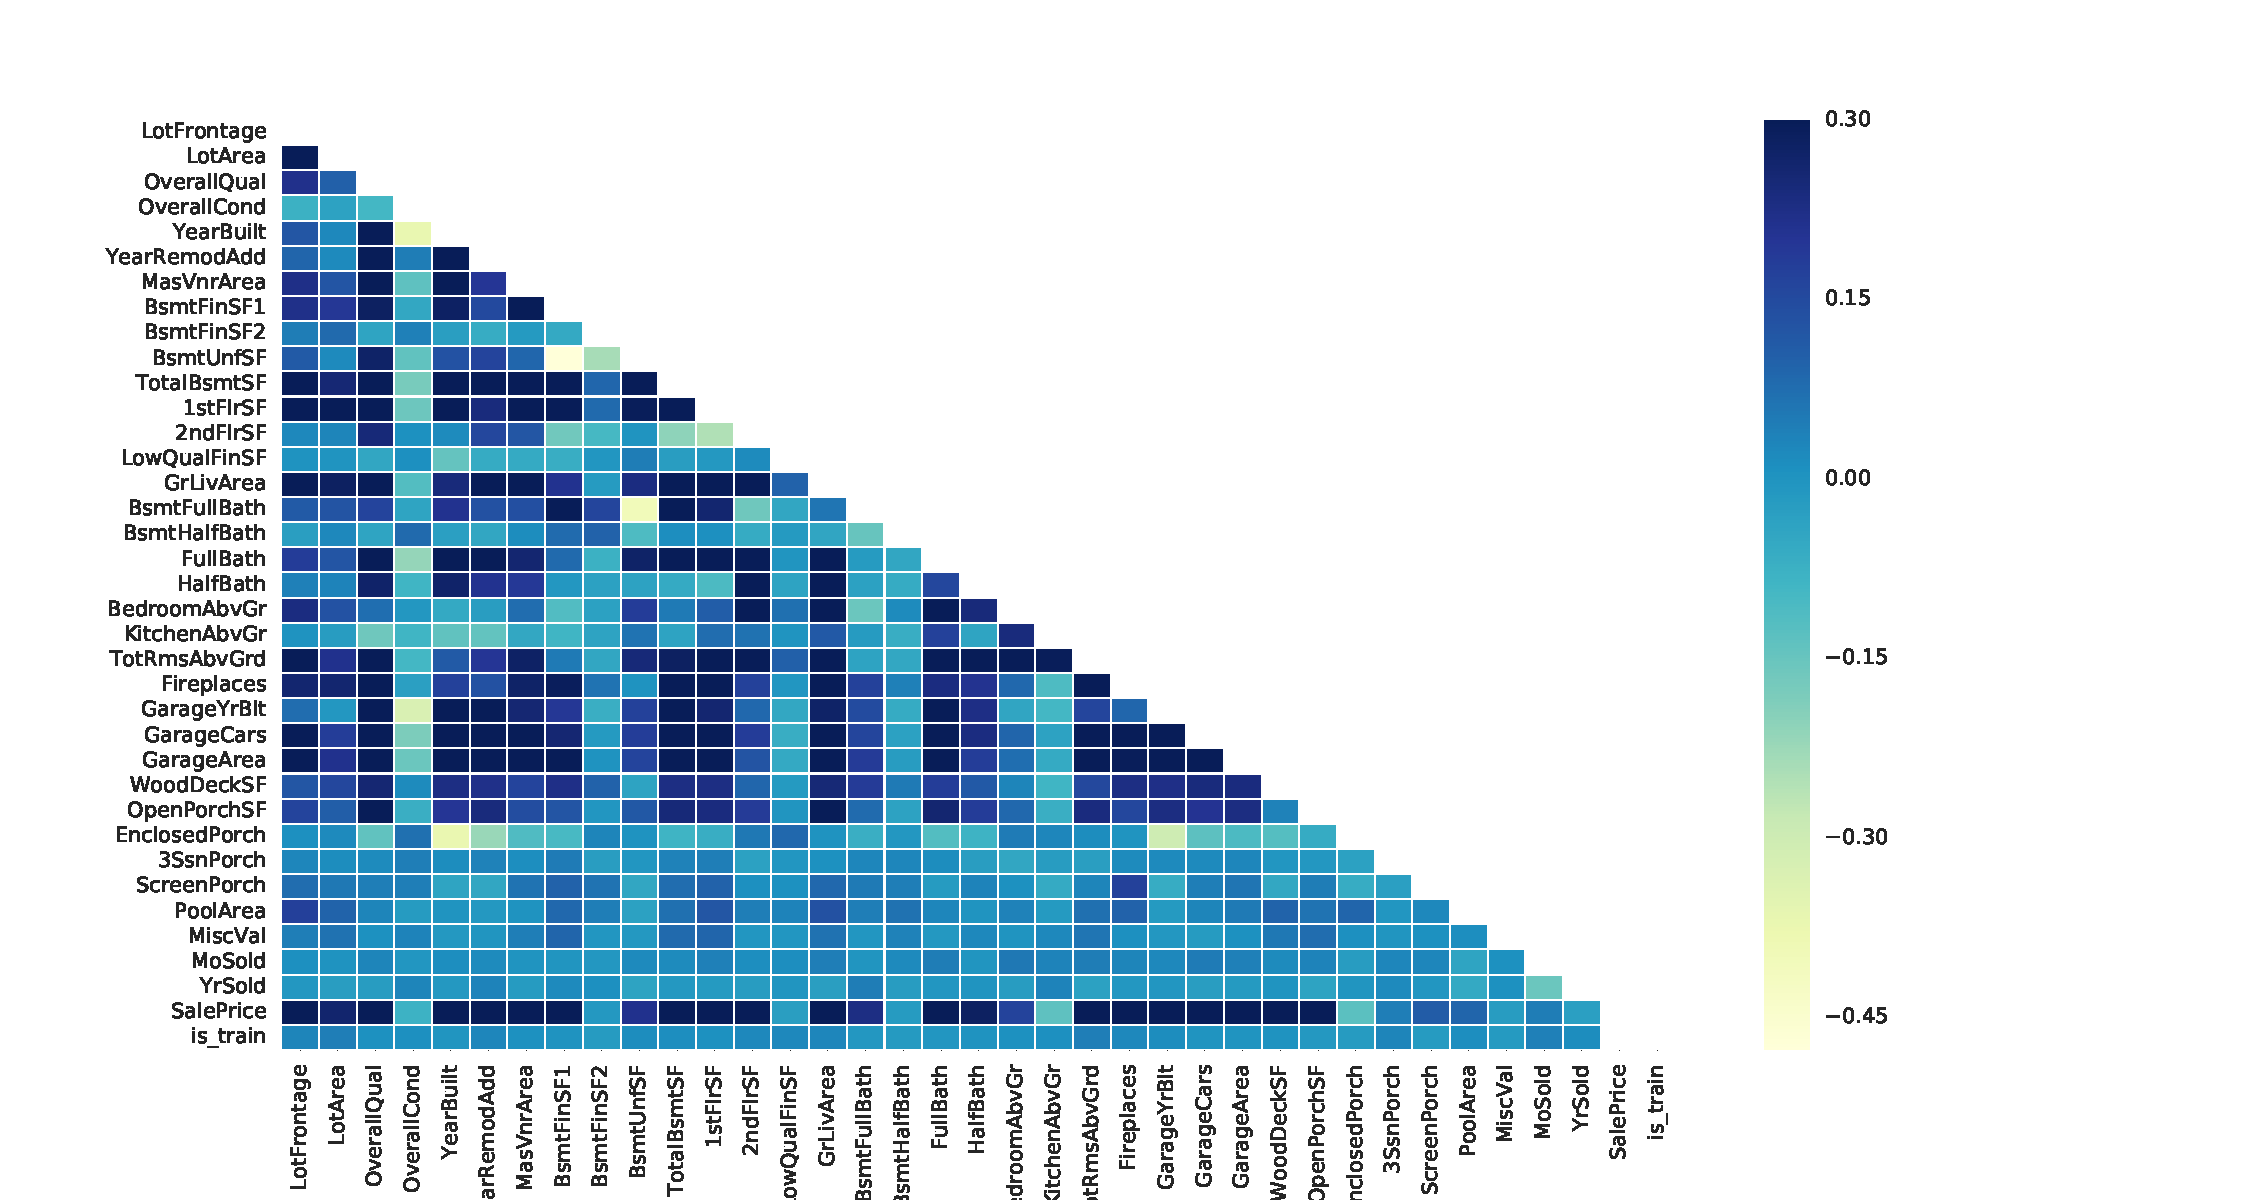
\includegraphics[width=0.99\columnwidth]{images/correlations}		
		\includegraphics[width=0.99\columnwidth]{images/pair-wise-correlations}
	\end{center}
	
	
	From the correlation plot we can visualize that there are 10 features strongly correlated with sale price. 
	
	\begin{enumerate}
		\item OverallQual: Overall material and finish quality
		\item GrLivArea: Above ground living area square feet
		\item GarageCars: Size of garage in car capacity
		\item GarageArea: Size of garage in square feet
		\item TotalBsmtSF: Total square feet of basement area
		\item 1stFlrSF: First Floor square feet
		\item FullBath: Full bathrooms above grade
		\item TotRmsAbvGrd: Total rooms above ground
		\item YearBuilt: Original construction date
		\item GarageYrBlt: Garage built year		
		
	\end{enumerate}
	
	Let us review Neighborhood category variable.
	
	\begin{lstlisting}[language=R]
	train_dat <- new_df[new_df$isTrain == 1, ]
	
	#sale price vs. Neighborhoods
	png("images/saleprice-vs-neighborhood.png", height=300)
	
	train_dat %>% select(Neighborhood, SalePrice) %>% 
	ggplot(aes(Neighborhood, SalePrice)) + 
	geom_boxplot() + 
	theme(axis.text.x = element_text(angle = 90, hjust =1)) + 
	xlab('Neighborhoods')
	
	dev.off()
	\end{lstlisting}
	
	\begin{center}
		\includegraphics[width=0.99\columnwidth]{images/saleprice-vs-neighborhood.png}	
		
	\end{center}
	
	\subsection{Handling Outliers}

	We will analyze the outliers using Cook's distance and then look at two key attributes - GrLiveArea and GarageArea that are in high correlation with Sale Price. Remove the outlier rows as they are only a few.
	
	\begin{lstlisting}[language=R]
	#*************************************
	#Dealing With Outliers
	#************************************
	#The variable GrLivArea and GarageArea are two variables with 
	#high correlation with SalePrice. Hence, it would be better 
	#to deal with the outliers for these variables
	
	nrow(new_df[new_df$isTrain == 1, ])
	train_dat <- new_df[new_df$isTrain == 1, ]
	
	test_dat <- new_df[new_df$isTrain == 0,]
	
	#*****************************************
	#handle outliers using Cook's distance
	#*****************************************
	
	formula <- as.formula(paste("SalePrice ~ ", paste(key_features, collapse="+")))
	
	outlier.model <- lm(formula = formula, data = train_dat)
	summary(outlier.model)
	
	#find outlier rows
	cooksd <- cooks.distance(outlier.model)
	
	# influential row numbers
	influential <- as.numeric(names(cooksd)[(cooksd > 4 * mean(cooksd, na.rm=T))])  
	
	key_features <- c(key_features, "SalePrice")
	
	#outlier rows
	nrow(train.clean[influential, key_features])
	png("images/outliers.png", height=300)
	outs <- influencePlot(outlier.model)
	dev.off()
	
	boxplot(train_dat$GrLivArea, main = "GrLivArea")
	
	boxplot(train_dat$GarageArea, main = "GarageArea")
	
	# Houses with garage area more 1200SF and grLivArea more than 4000SF are removed because they are gargantuan and their presence is adding skewness to the data.
	
	#find and remove outlier rows
	outlier_rows <- c(which(train$GarageArea > 1200),
	which(train$GrLivArea >=  4000))
	
	train_dat <- train_dat[-outlier_rows, ]
	
	#Outliers are also removed from our response variable
	y_true <- train$SalePrice[-outlier_rows]
	\end{lstlisting}
	
	\begin{center}
		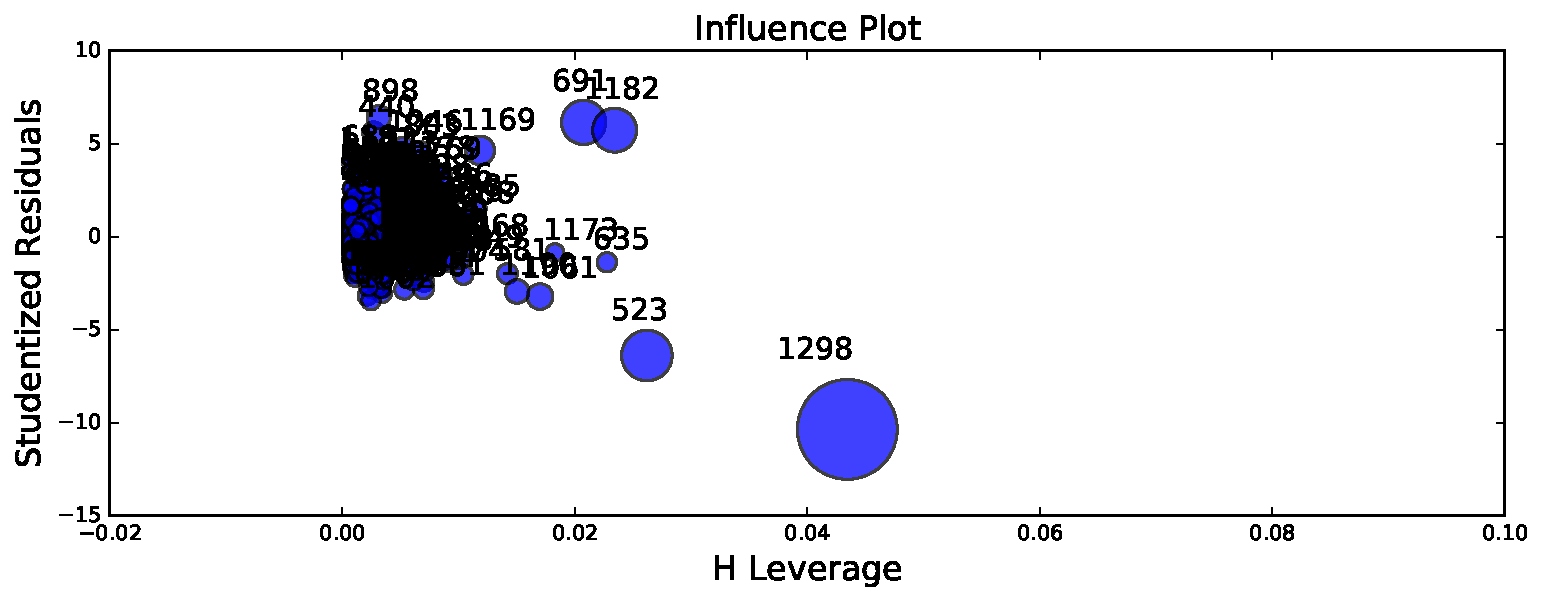
\includegraphics[width=0.99\columnwidth]{images/outliers}		
		\includegraphics[width=0.99\columnwidth]{images/GrLivArea2}		
		\includegraphics[width=0.99\columnwidth]{images/GarageArea2}
	\end{center}
	
	
	
	\subsection{Addressing Skewed Data}

	Let us visualize the skewed data with skewness $>$ 50\%. We will adjust only the Sale Price to the corresponding LOG value - LOG(SalePrice + 1).
	
	\begin{lstlisting}[language=R]
	#***********************************************
	# handle skewed numeric data
	#************************************************
	
	#We will only transform variables that are 'moderate' to 'highly' skewed. 
	#We will also only transform non-categorical variables.
	#skwed data
	
	skewedVars <- c("SalePrice")
	y_train <-log(y_true+1)
	
	train_dat_names <- names(train_dat)
	
	for(i in key_features){
	if(is.element(i, train_dat_names)){
	if(abs(skewness(train_dat[,i])) > 0.5){
	skewedVars <- c(skewedVars, i)
	}}}
	
	png("images/skewed-SalePrice.png", height=200)
	par(mfrow = c(1,2))
	plot(density(y_true), main = "SalePrice")
	plot(density(y_train), main = paste("Log(SalePrice + 1)", sep = ""))
	dev.off()
	
	#remove SalePrice
	skewedVars <- skewedVars[-1]
	
	#plot graphs - actual and logarithmic values of the key skewed attributes only
	for(i in 1:length(skewedVars)){
	print(skewedVars[i]);
	png(paste0("images/skewed-",skewedVars[i], ".png"), height=200)
	
	par(mfrow = c(1,2))
	plot(density(train_dat[,skewedVars[i]]), main = skewedVars[i])
	plot(density(log(train_dat[,skewedVars[i]] + 1)), main = paste("Log(", skewedVars[i], " + 1)", sep = ""))
	dev.off()
	}
	
	#we dont need to adjust the other variables
	#for(i in skewedVars){
	#  if(0 %in% train_dat[, i]){
	#    train_dat[,i] <- log(1 + train_dat[,i])
	#  }
	#  else{
	#    train_dat[,i] <- log(train_dat[,i])
	#  }
	#}
	
	\end{lstlisting}
	
	\begin{center}	
		
		\includegraphics[width=0.99\columnwidth]{images/skewed-SalePrice}		
		\includegraphics[width=0.99\columnwidth]{images/skewed-GrLivArea}
		\includegraphics[width=0.99\columnwidth]{images/skewed-X1stFlrSF}		
		\includegraphics[width=0.99\columnwidth]{images/skewed-TotRmsAbvGrd}
		\includegraphics[width=0.99\columnwidth]{images/skewed-YearBuilt}
	\end{center}
	
	
	
	%----------------------------------------------------------------------------------------
	% Algorithm and Methodology
	%----------------------------------------------------------------------------------------
	\section{Algorithm and Methodology}

	As per the given assignment, we will do the simple linear regression and then compare the accuracy with a few other algorithms in the following sections.
	
	\subsection{Principal Component Analysis (PCA)}
	
	Simple linear regression will not effectively work with too many attributes in the model. We will use {\em principle component analysis (PCA)} to identify the principal - key attributes.
	
	\begin{lstlisting}[language=R]
	ds.pca <- prcomp(train_dat[,num_features], scale =TRUE)
	summary(ds.pca)
	
	png("images/pca.png", height=300)
	#scree plot to identify how many principal components
	plot(ds.pca, type = "l", ylim=c(0, 10), main="PCA")
	dev.off()
	\end{lstlisting}
	
	\begin{center}		
		\includegraphics[width=0.99\columnwidth]{images/pca}	
	\end{center}
	
	\subsection{Linear Regression}
		
	We will create simple linear regression model with two principle components - OverallQual and GrLivArea to train the model.
	
	\begin{lstlisting}[language=R]
	pca_features <- c("OverallQual","GrLivArea")
	
	formula <- as.formula(paste("SalePrice ~ ", paste(pca_features, collapse="+")))
	
	linear_data = cbind(train_dat, SalePrice = y_train)
	
	linearModel <- lm(formula, data=linear_data)
	summary(linearModel)
	
	prediction <- predict(linearModel, test_dat)
	linearPreds <- data.frame(Id = test['Id'], SalePrice= prediction)
	
	SSE <- sum((y_train - prediction) ^ 2)
	SST <- sum((y_train - mean(y_train)) ^ 2)
	error <- (1 - SSE/SST)
	
	#make sure there are no -ve values for SalePrice
	wrongPredictions <- linearPreds[linearPreds$SalePrice <= 0,]
	if (nrow(wrongPredictions) = 0){
	#we are good to go
	write.csv(linearPreds, "simple.linear.submission.csv", row.names = F)
	}
	
	\end{lstlisting}
	
	Adjusted R-squared of 0.7689 tells us that approximately 76\% of variation in sale price can be explained by this model. F-statistics and p-value show the overall significance test of the model.
	%----------------------------------------------------------------------------------------
	% Experiments and Results
	%----------------------------------------------------------------------------------------
	\section{Experiments and Results}
	
	
	The Kaggle score for the simple linear regression is pretty bad (5.55). After reviewing a few models created by other Kaggle developers, it is evident that we need to try more advanced regression models.
	For this assignment, we will examine better regression algorithms such as, XGB boosting, Random Forest, Ridge, Lasso and Elastic Net. All these algorithms do cross-validation such as 5 folds or 10 folds from training data set and provide a commonly used trade-off between speed of compute time and generalize error estimate. In the end we will conclude it with ensembled result set from best of the three to four algorithms.
	
	\subsection{Feature Engineering}

	Before we continue to the advanced regression models, let us do some feature engineering by creating a few new attributes from existing attributes. We have created 5 new attributes - TotalSqFt, TotalBaths, Remodeled, RecentRemodel, and NewHouse. We have also removed the rows of having no variance.
	
	\begin{lstlisting}[language=R]
	#************************************
	# feature engineering
	#**************************************
	# new columns
	
	numeric_dat['TotalSqFt'] <-  comb_data$GrLivArea + comb_data$TotalBsmtSF
	numeric_dat['TotalBaths'] <-  comb_data$BsmtFullBath + comb_data$FullBath + (0.5 * (comb_data$BsmtHalfBath + comb_data$HalfBath))
	
	## New column when the house was not remodeled in the same year as built
	
	numeric_dat['Remodeled'] <- (comb_data$YearBuilt != comb_data$YearRemodAdd) * 1
	
	numeric_dat['RecentRemodel'] <- (comb_data$YearRemodAdd >= comb_data$YrSold) * 1
	
	#New column for house sold in the same year it was built
	
	numeric_dat['NewHouse'] <- (numeric_dat$YearBuilt == numeric_dat$YrSold) * 1
	
	
	#**************************************************
	#Variables showing near zero variance
	
	nzv_logic <- nearZeroVar(df, saveMetrics = TRUE)
	
	nzv_var <- rownames(nzv_logic)[nzv_logic$nzv==TRUE]
	
	new_df <- df[,!names(df) %in% nzv_var]
	
	#Dimensions of the feature engineered dataset
	dim(new_df)
	\end{lstlisting}
	
	
	
	\subsection{XGB Boosting}

	Gradient boosting models (GBM) are one of the most popular algorithms on Kaggle. A variant of GBMs known as the XGBoost has been a clear favorite for many recent competitions. The algorithm works well right out of the box. It is a type of ensemble model, like the random forest, where multiple decision trees are used and optimized over some cost function. To simplify the feature selection process, we fitted a {\em XGBoost} model containing all of the housing features to determine the most important predictors of SalePrice. XGBoost efficiently sorts each of the housing features by its {\em Fscore}, which is a measure of variable importance. 
	
	\begin{lstlisting}[language=R]
	#****************************************************
	#XGBoosting were used for predicting the housing prices.
	
	#XGBoost has its own function to create matrix for the modeling
	
	dtrain <- xgb.DMatrix(as.matrix(train_dat), label = y_train)
	dtest <- xgb.DMatrix(as.matrix(test_dat))
	
	
	cv.ctrl <- trainControl(method = "repeatedcv", repeats = 1,number = 4, 
	allowParallel=T)
	
	xgb.grid <- expand.grid(nrounds = 750,
	eta = c(0.01,0.005,0.001),
	max_depth = c(4,6,8),
	colsample_bytree=c(0,1,10),
	min_child_weight = 2,
	subsample=c(0,0.2,0.4,0.6),
	gamma=0.01)
	
	set.seed(1234)
	
	xgb_tune <- train(as.matrix(train_dat),
	y_train, method="xgbTree", 
	trControl=cv.ctrl, 
	tuneGrid=xgb.grid, 
	verbose=T, metric="RMSE", nthread =3)
	
	xgb_params <- list(
	booster = 'gbtree',
	objective = 'reg:linear',
	colsample_bytree=1,
	eta=0.01,
	max_depth=8,
	min_child_weight=3,
	alpha=0.3,
	lambda=0.4,
	gamma=0.01, # less overfit
	subsample=0.4,
	seed=5,
	silent=TRUE)
	
	bst <- xgb.train(xgb_params,dtrain, nrounds = 10000, early_stopping_rounds = 300, watchlist = list(train=dtrain))
	
	#To test how well the model has done the RMSE value is calculated.
	
	# Functtion to calculate the RMSE value
	rmse_eval <- function(y.true, y.pred) {
	mse_eval <- sum((y.true - exp(y.pred)-1)^2) / length(y.true)
	return(sqrt(mse_eval))
	}
	
	y_pred.xgb <- predict(bst, dtrain)
	rmse_eval(y_true, y_pred.xgb)
	
	#feature ranking
	model.names <- dimnames(train_dat)[[2]]
	
	importance_matrix <- xgb.importance(model.names, model = bst)
	
	png("images/xgb-feature-ranking.png", height=300)
	#Plotting 10 most important feature that contribute to the model
	xgb.plot.importance(importance_matrix[1:10])
	dev.off()
	
	pred.xgb <- predict(bst, as.matrix(test_dat))
	
	xgb.SalePrice <- as.data.frame(exp(pred.xgb)-1)
	
	colnames(xgb.SalePrice) <- c("1")
	
	PredictedPrice <- cbind(test['Id'], xgb.SalePrice)
	colnames(PredictedPrice) <- c("Id", "SalePrice")
	
	#make sure there are no -ve values for SalePrice
	wrongPredictions <- PredictedPrice[PredictedPrice$SalePrice <= 0,]
	if (nrow(wrongPredictions) == 0){
	#we are good to go
	write.csv(PredictedPrice, file = "xgb.submission.csv", row.names = F)
	}
	\end{lstlisting}
	
	\begin{center}		
		\includegraphics[width=0.99\columnwidth]{images/xgb-feature-ranking}	
	\end{center}
	
	\subsection{Random Forest}

	A more advanced model, the random forest uses multiple decision trees and gives the mean prediction of each tree. This is somewhat of a black box approach as the random forest mechanism is not very clear as it will give model results, but lack information on coefficients which is something we normally get from an output of a regression model. However, Random forest has a nice feature ranking functionality.
	
	\begin{lstlisting}[language=R]
	#**************************************
	#Random forest 
	#*************************************
	
	model_rf <- randomForest(y_train ~ ., data = train_dat, importance = T)
	
	#get feature ranking to compare with XGB
	
	# Variable importance of the latest model
	importance    <- importance(model_rf)
	varImportance <- data.frame(Variables = row.names(importance), 
	Importance = round(importance[ ,'%IncMSE'],2))
	
	# Create a rank variable based on importance
	rankImportance <- varImportance  %>% mutate(Rank = dense_rank(desc(Importance)))
	rankImportance[order(rankImportance$Rank),] 
	
	rankImportance <- rankImportance[which(rankImportance$Rank <= 10),]
	rankImportance[order(rankImportance$Rank), -c(2)] 
	
	# Use ggplot2 to visualize the relative importance of variables
	print("Variable importance")
	
	png("images/rf-feature-ranking.png")
	ggplot(rankImportance, aes(x = reorder(Variables, Importance), 
	y = Importance, fill = Importance)) +
	geom_bar(stat='identity') + 
	geom_text(aes(x = Variables, y = 0.5, label = Rank),
	hjust=0, vjust=0.55, size = 4, colour = 'red') +
	labs(x = 'Variables') +
	coord_flip() + theme_few()
	
	dev.off()
	
	
	pred.rf <- predict(model_rf, test_dat)
	rf.SalePrice <- as.data.frame(exp(pred.rf)-1)
	
	PredictedPrice <- cbind(test['Id'], rf.SalePrice)
	colnames(PredictedPrice) <- c("Id", "SalePrice")
	#make sure there are no -ve values for SalePrice
	wrongPredictions <- PredictedPrice[PredictedPrice$SalePrice <= 0,]
	
	if (nrow(wrongPredictions) == 0){
	#we are good to go
	write.csv(PredictedPrice, file = "rf.submission.csv", row.names = F)
	}
	\end{lstlisting}
	
	\begin{center}		
		\includegraphics[width=0.99\columnwidth]{images/rf-feature-ranking}	
	\end{center}
	
	List of top 10 attributes that influence SalePrice from Random Forest algorithm:
	
	\begin{lstlisting}[language=R]
	Attribute      Rank
	
	TotalSqFt       1
	OverallQual     2
	LotArea         3
	GrLivArea       4
	OverallCond    	5
	GarageArea      6	
	BsmtFinSF1	    7
	YearBlt         8
	TotalBaths      9
	TotalBsmtSF    10
	\end{lstlisting}
	
	\subsection{Ridge, LASSO, Elastic Network and Ensemble}
	
	One limitation of XGBoost algorithm, in particular, is its inability to extrapolate and because of this linear model can better predict any sale prices outside the range of prices given in our training set. Hence, regularized linear models are used with penalty term lambda to minimize the error. LASSO, also known as Least Absolute Shrinkage and Selection Operator, is a regression model that does variable selection and regularization. The LASSO model uses a parameter that penalizes fitting too many variables. It allows the shrinkage of variable coefficients to 0, which essentially results in those variables having no effect in the model, thereby reducing dimensionality. Let us work on Ridge, LASSO and Elastic Net regularizations using GLMNET package to predict the SalePrice. We will take four best algorithms based on Kaggle Score to create the ensembled prediction to get better score in the Kaggle submissions. 
	
	\begin{lstlisting}[language=R]
	#*****************************************
	# Ridge, LASSO, Net
	#***************************************
	#For regularization, a matrix is generated
	
	x <- train_dat %>% data.matrix()
	
	# a range of lambdas are generated over which regularization can be tested
	lamdas <- 10^seq(3, -2, by = -.1)
	
	#cv.glm net provides the optimum lambda for regularization
	#nfolds = 10 cross validation sets
	
	#Does k-fold cross-validation for glmnet, produces a plot, and returns a value for lambda
	
	glm.cv.ridge <- cv.glmnet(x, y_train, alpha = 0, lambda = lamdas, nfolds = 10)
	glm.cv.lasso <- cv.glmnet(x, y_train, alpha = 1, lambda = lamdas, nfolds = 10)
	glm.cv.net <- cv.glmnet(x, y_train, alpha = 0.01, lambda = lamdas, nfolds = 10)
	
	png("images/lamda.png", height=300)
	par(mfrow=c(1,3))
	
	plot(glm.cv.ridge, main = "Ridge")
	plot(glm.cv.lasso, main = "Lasso")
	plot(glm.cv.net, main = "Elastic Net")
	
	dev.off()
	
	#The the minimum value is optimum lambda 
	penalty.ridge <- glm.cv.ridge$lambda.min
	penalty.lasso <- glm.cv.lasso$lambda.min
	penalty.net <- glm.cv.net$lambda.min
	
	
	pred.ridge <- predict(glm.cv.ridge, s = penalty.ridge, newx = data.matrix(test_dat))
	ridge.SalePrice <- as.data.frame(exp(pred.ridge)-1)
	
	PredictedPrice <- cbind(test['Id'], ridge.SalePrice)
	colnames(PredictedPrice) <- c("Id", "SalePrice")
	
	#make sure there are no -ve values for SalePrice
	wrongPredictions <- PredictedPrice[PredictedPrice$SalePrice <= 0,]
	
	if (nrow(wrongPredictions) == 0){
	#we are good to go
	write.csv(PredictedPrice, file = "ridge.submission.csv", row.names = F)
	}
	
	pred.lasso <- predict(glm.cv.lasso, s = penalty.lasso, newx = data.matrix(test_dat))
	lasso.SalePrice <- as.data.frame(exp(pred.lasso)-1)
	
	PredictedPrice <- cbind(test['Id'], lasso.SalePrice)
	colnames(PredictedPrice) <- c("Id", "SalePrice")
	
	#make sure there are no -ve values for SalePrice
	wrongPredictions <- PredictedPrice[PredictedPrice$SalePrice <= 0,]
	
	if (nrow(wrongPredictions) == 0){
	#we are good to go
	write.csv(PredictedPrice, file = "lasso.submission.csv", row.names = F)
	}
	
	pred.net <- predict(glm.cv.net, s = penalty.net, newx = data.matrix(test_dat))
	net.SalePrice <- as.data.frame(exp(pred.net)-1)
	
	PredictedPrice <- cbind(test['Id'], net.SalePrice)
	colnames(PredictedPrice) <- c("Id", "SalePrice")
	
	#make sure there are no -ve values for SalePrice
	wrongPredictions <- PredictedPrice[PredictedPrice$SalePrice <= 0,]
	
	if (nrow(wrongPredictions) == 0){
	#we are good to go
	write.csv(PredictedPrice, file = "net.submission.csv", row.names = F)
	}
	
	\end{lstlisting}
	
	\begin{center}		
		\includegraphics[width=0.99\columnwidth]{images/lambda}	
	\end{center}
	
	\subsection{Ensemble Models}
	Predictions from XGB, Random Forest, Ridge, LASSO and Elastic Network are submitted to Kaggle and the top four scores are from XGB, Ridge, LASSO and Elastic Network. Random Forest score was lesser compared to these four algorithms for this data set. Following are the Kaggle Scores for these algorithms from our submissions.
	
	\begin{lstlisting}[language=R]
	Algorithm                    Kaggle Score
	
	Elastic Net                     0.12510
	LASSO Regression                0.12899
	XGB Boosting                    0.13018
	Ridge Regression                0.13766
	Random Forest                   0.21256
	Simple Linear Regression        5.52
	\end{lstlisting}
	
	We will ensemble the SalePrice predictions using the predicted sale prices of top 4 performing algorithms - Elastic Net, LASSO, XGB and Ridge, and submit the SalePrice predictions to Kaggle.
	
	\begin{lstlisting}[language=R]
	SalePrice <- (xgb.SalePrice + ridge.SalePrice + lasso.SalePrice + net.SalePrice)/4.0
	
	PredictedPrice <- cbind(test['Id'], SalePrice$`1`)
	
	colnames(PredictedPrice) <- c("Id", "SalePrice")
	
	write.csv(PredictedPrice, file = "ensemble.submission.csv", row.names = F)
	
	\end{lstlisting}
	
		%----------------------------------------------------------------------------------------
	% Summary and Conclusions
	%----------------------------------------------------------------------------------------
	\section{Summary and Conclusions}
		
	As expected the ensemble result set got better score (0.12014) in Kaggle submissions. Following is the list of Kaggle Scores from the algorithms that we have tried.
	
	\begin{center}
		\includegraphics[width=0.6\columnwidth]{submissions/kaggle_scores}
	\end{center}
	
	\nocite{*}
	
	\begin{acks}	
			The authors would like to thank Dr. Gregor von Laszewski and the Teaching Assistants for their support and valuable suggestions. Authors would like to thank Kaggle Website and the developers for their valuable information, ideas and contributions.		
	\end{acks}


	\bibliographystyle{ACM-Reference-Format}
	\bibliography{report} 	

	
\end{document}
